\section{Implementierung der robusten Spielererkennung}
\abschnittsautor{M. Ishak}

Dieser Abschnitt dokumentiert die praktische Umsetzung der Computer-Vision-Pipeline. Der Fokus liegt 
dabei auf der Erstellung eines verdeckungstoleranten Datensatzes, dem Fine-Tuning der YOLOv8-Modelle 
sowie der Konstruktion einer geometrisch korrekten Schnittstelle für das anschließende Kamera-Tracking.

\subsection{Datenbeschaffung und Annotation}
Erste Evaluierungen mit dem vortrainierten Standard-Modell von YOLOv8 (ohne Fine-Tuning) zeigten 
deutliche Schwächen im fußballspezifischen Kontext. Insbesondere bei Verdeckungen (Occlusion) 
traten hohe Fehlerquoten auf, und Spieler wurden vom Basismodell teilweise fälschlicherweise als 
irrelevante Objekte (beispielsweise als Fahrräder) klassifiziert. Um diese Defizite zu beheben, 
wurde ein domänenspezifischer Datensatz konstruiert.

Der finale Datensatz setzt sich aus zwei Quellen zusammen: Um eine hohe Grundvarianz an Spielsituationen, 
Lichtverhältnissen und Trikotfarben zu gewährleisten, wurden rund 10.000 bereits öffentlich zugängliche 
Bilder von der Plattform Roboflow integriert. Um das Modell jedoch gezielt auf die spezifische Perspektive 
und Verdeckungssituationen des Projekts zu trainieren, wird dieser Stamm-Datensatz um 100 bis 500 eigens 
erstellte Bilder erweitert. Diese Aufnahmen bestehen aus extrahierten Screenshots von YouTube-Videos, 
Bildmaterial von Fußballvereinen sowie verschiedenen Online-Quellen. Zusätzlich sind eigene Videoaufnahmen 
von Amateurspielen (aufgenommen mit einem iPhone 15 Pro) eingeplant, um die exakte Kameraposition des Projekts 
zu simulieren.

Die Annotation des gesamten Datensatzes erfolgte auf der Plattform Roboflow. Es wurden vier Zielklassen 
definiert: \texttt{player}, \texttt{goalkeeper}, \texttt{referee} und \texttt{ball}. Um den Arbeitsaufwand 
bei der Markierung des Balls zu minimieren, kam das KI-gestützte Segmentierungswerkzeug \ac{SAM} 
(Segment Anything Model) von Roboflow zum Einsatz. Die Spieler wurden hingegen manuell mit Bounding 
Boxes versehen. Dabei wurde strikt das Prinzip der \textit{Amodal Bounding Box} angewendet: Die Begrenzungsbox
wurde vom Kopf des Spielers bis exakt zu dem Punkt gezogen, an dem die Füße den Rasen berühren -- selbst dann, 
wenn die Beine durch einen Gegenspieler verdeckt waren. Diese Methodik ist zwingend erforderlich, um dem 
nachfolgenden Homografie-Modul stets die korrekte Bodenkoordinate für die 2D-Transformation zu liefern.


 \begin{figure}[htbp]
     \centering
     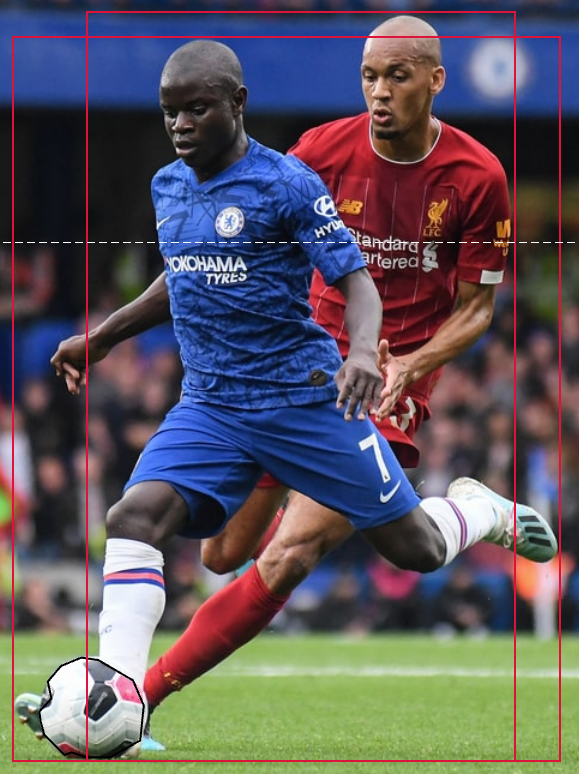
\includegraphics[width=0.75\linewidth]{images/roboflow-amodal-ishak.png}
     \caption{Annotation in Roboflow: Die Bounding Box wird bis zur Rasenebene gezogen (Amodal Bounding Box), um den Fußpunkt für das Tracking zu sichern.}
     \label{abb:roboflow-amodal}
 \end{figure}

\subsection{Setup der Trainingsumgebung und Hardware}
Die Aufnahme der realen Spieldaten erfolgt über ein Zwei-Kamera-Setup, dessen Bilder zu einem nahtlosen 
Panorama zusammengefügt werden. Dies stellt sicher, dass Spieler beim Verlassen eines einzelnen Kamerabildes 
nicht aus dem Frame verschwinden und das Tracking nicht abbricht. 

Für die Softwareentwicklung und das Modell-Training wurde die Arbeitslast auf zwei unterschiedliche 
Hardware-Systeme aufgeteilt. Ein MacBook Pro (mit Apple M1 Chip) fungiert als primäre Entwicklungsstation. 
Hier werden die Datensätze in Roboflow annotiert, die theoretische Dokumentation verfasst und der Python-Code 
für die Inferenz geschrieben. Da der M1-Chip für das Deep-Learning-Training großer Modelle über hunderte 
Epochen jedoch nicht die erforderliche Rechenleistung aufweist, wurde das eigentliche Fine-Tuning ausgelagert.

Das rechenintensive Modell-Training, die Fehleranalyse und die Code-Kompilierung für das neuronale Netz werden 
auf einem dedizierten Windows-PC mit einer NVIDIA RTX 3080 Grafikkarte durchgeführt. Die hohe Anzahl an 
CUDA-Cores und der große VRAM (Video Random Access Memory) dieser GPU reduzieren die Trainingsdauer signifikant.

Die Synchronisation des Quellcodes und der Dokumentation im Team erfolgt über die Versionsverwaltung Git 
und die Plattform GitHub. Während die schriftliche Dokumentation in einem gemeinsamen Team-Repository gepflegt 
wird, wurde für das Training der Künstlichen Intelligenz ein separates, privates GitHub-Repository eingerichtet.
Dort werden die Trainingsskripte, Konfigurationsdateien und schließlich die fertigen Modellgewichte (Weights) 
hochgeladen, sodass die fertige KI nach Abschluss des Trainings von jedem System aus heruntergeladen und für 
die Inferenz genutzt werden kann.

\subsection{Fine-Tuning und Hyperparameter-Konfiguration}
Für das Training des Modells fiel die Wahl primär auf die Architektur YOLOv8-Nano (\texttt{yolov8n.pt}), 
mit der Option einer späteren Skalierung auf YOLOv8-Small (\texttt{yolov8s.pt}). Diese Entscheidung basiert 
auf einem Kompromiss zwischen der maximalen Inferenzgeschwindigkeit -- welche für die spätere Videoanalyse 
unerlässlich ist -- und der Speicherkapazität (VRAM) der lokal verwendeten NVIDIA RTX 3080.

Das Fine-Tuning wurde initial über 50 Epochen mit einer Batch-Size von 16 angesetzt. Als Grundlage dient ein 
kombinierter Datensatz aus etwa 1.500 Aufnahmen. Da das zu analysierende Videomaterial über ein 
Zwei-Kamera-Setup aus knapp fünf Metern Höhe in 4K-Auflösung aufgezeichnet wird, ist die Wahl der 
Eingangsauflösung (\texttt{imgsz}) kritisch. Während erste Trainingsläufe und Validierungen auf 640 Pixel 
normiert wurden (siehe Quellcode~\ref{code:training}), erfordern die feinen Details des Panoramabildes in 
der finalen Evaluierung höhere Auflösungen.

\begin{lstlisting}[language=Python, caption={Initiales Trainings-Skript für das YOLOv8 Fine-Tuning}, label=code:training]
from ultralytics import YOLO

if __name__ == "__main__":
    model = YOLO("yolov8n.pt")
    
    model.train(
        data="C:/vertex-ki/dataset/data.yaml",
        epochs=50,
        imgsz=640,
        device=0,
        batch=16,
        project="runs/train",
        name="fussball_v1"
    )
\end{lstlisting}

\subsection{Optimierung der Inferenz für Verdeckung (Occlusion)}
Die erste Trainingsphase dient primär der Identifikation von Modellschwächen, insbesondere bei extremen 
Spielerdichten im Strafraum. Um zu verhindern, dass die \ac{NMS} (Non-Maximum Suppression) gültige Spieler 
bei Überschneidungen fälschlicherweise löscht, wird in der Inferenz-Phase der \ac{IoU}-Schwellenwert 
situationsbedingt angepasst.

Da das breite 4K-Panoramabild die Spieler auf der gegenüberliegenden Spielfeldseite extrem klein darstellt, 
wird zusätzlich der \ac{SAHI}-Algorithmus (Slicing Aided Hyper Inference)~\cite{akyon2022sahi} in die Pipeline integriert. Dieses 
Verfahren zerschneidet das großflächige Quellbild in kleinere, überlappende Kacheln (Slices). Das YOLO-Modell 
inferiert jede Kachel separat in voller Auflösung, bevor die erkannten Bounding Boxes über ein angepasstes 
NMS-Verfahren wieder zum Gesamtbild zusammengefügt werden. Diese Methode steigert die Erkennungsrate (Recall) 
bei kleinen und teilweise verdeckten Spielern massiv, ohne dass das Modelltraining auf unrealistisch hohe 
Auflösungen skaliert werden muss.

\subsection{Entwicklung der Datenschnittstelle (JSON-Export)}
Um die erkannten Bildkoordinaten an das nachfolgende Modul zur Homografie-Berechnung zu übergeben, wurde 
eine entkoppelte Datenschnittstelle konzipiert. YOLO exportiert Bounding Boxes nativ in einem normierten Format,
bestehend aus Klassen-ID, dem Zentrum der Box ($x_{center}, y_{center}$) sowie der relativen Breite und Höhe
(siehe Quellcode~\ref{code:yolo-labels}). 

\begin{lstlisting}[caption={Auszug aus den nativen YOLO-Label-Daten (Klassen-ID, x\_center, y\_center, width, height)}, label=code:yolo-labels]
2 0.5201979 0.3360462 0.0223489 0.0405833
2 0.5638020 0.2935185 0.0130208 0.0370370
1 0.7028645 0.2861111 0.0109375 0.0388888
\end{lstlisting}

Da das Zentrum der Bounding Box anatomisch den Torso des Spielers abbildet, würde eine direkte 2D-Transformation
aufgrund der Kameraperspektive zu erheblichen Parallaxenfehlern auf dem virtuellen Spielfeld führen. Ein 
eigens entwickeltes Python-Skript konvertiert daher diese normierten Daten in absolute Pixelkoordinaten und 
berechnet den exakten Fußpunkt auf der Rasenebene. Da YOLO das obere linke Eck des Bildes als Ursprung $(0,0)$ 
definiert, ergibt sich die absolute Y-Koordinate des Fußpunktes ($y_{foot}$) mathematisch aus 
$y_{center} + \frac{height}{2}$. 

Die bereinigten Daten werden Frame für Frame in einer strukturierten JSON-Datei gespeichert. Diese enthält 
die Frame-Nummer, die Klassen-ID (0: ball, 1: goalkeeper, 2: player, 3: referee), den Confidence-Score sowie 
die korrigierten Fußpunkt-Koordinaten (X und Y) in Pixeln. Dieser strukturierte JSON-Export dient als robuster 
Datenvertrag (Data Contract) für die anschließende Distanzberechnung und das Dashboarding.